\documentclass[assd_guia_filtros_recursivos_main.tex]{subfiles}


\begin{document}

\section*{Ejercicio 4}

\subsection*{4.a}
\begin{equation}
	H(s) = \frac{8}{ (s+2)\cdot(s+4) }
\end{equation}

\begin{equation}
	H(z) = \frac{4\cdot \left( e^{-2T} - e^{-4T} \right) \cdot z}
	{z^2 - \left( e^{-2T} + e^{-4T} \right)\cdot z + e^{-6T}}
\end{equation}

\begin{figure}[htbp]
	\centering
	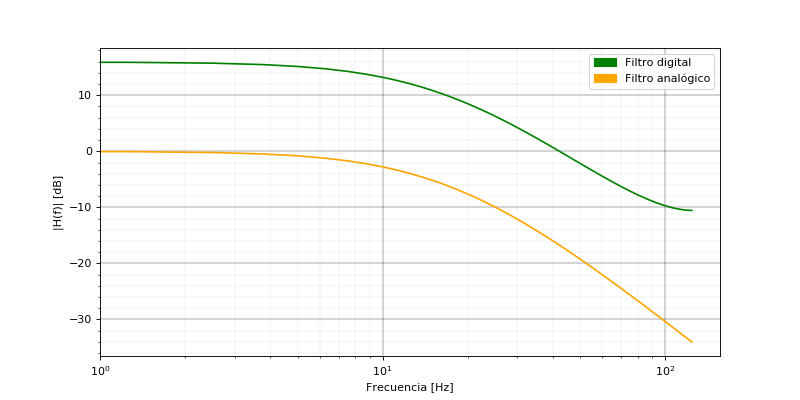
\includegraphics[width=\textwidth]
	{ej4_a.png}
	\caption{M\'etodo invariante al impulso (ejercicio 4.a)}
\end{figure}

\subsection*{4.b}
\begin{equation}
	H(s) = \frac{8}{ s\cdot(s+2)\cdot(s+4) }
\end{equation}

\begin{equation}
	H(z) = \frac
	{z \cdot \left[ 	\left( 1-2e^{-2T}+e^{-4T} \right) \cdot z 
	+ e^{-6T} -2e^{-4T} +e^{-2T}		\right]}
	{z^3 - \left( 1+e^{-2T}+e^{-4T} \right) \cdot z^2 +
	 \left( e^{-2T}+e^{-4T} +e^{-6T} \right) \cdot z- e^{-6T}}
\end{equation}

\begin{figure}[htbp]
	\centering
	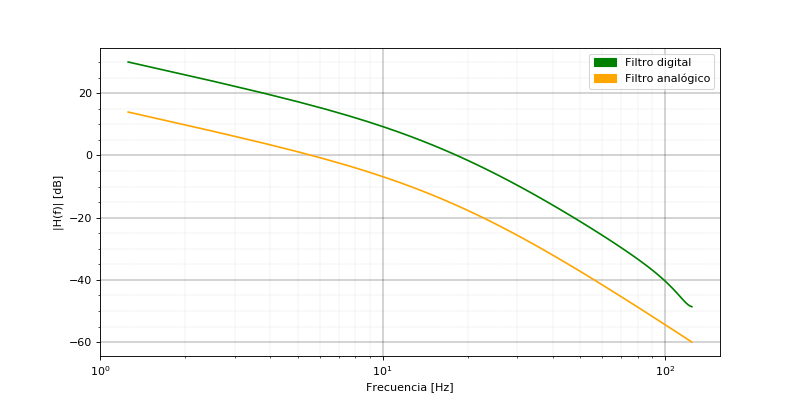
\includegraphics[width=\textwidth]
	{ej4_b.png}
	\caption{M\'etodo invariante al impulso (ejercicio 4.b)}
\end{figure}

\subsection*{4.c}

\begin{equation}
	H(s) = \frac{s+1}{(s+0.5)\cdot (s+4)}
\end{equation}

\begin{equation}
	H(z) = \frac
	{
		z\cdot \left[ z - \frac{1}{7}\cdot (e^{-4T}+6e^{-\nicefrac{T}{2}}) \right]
	}
	{
		z^2 - (e^{-4T}+e^{-\nicefrac{T}{2}})\cdot z + e^{-\nicefrac{9T}{2}}
	}
\end{equation}

\begin{figure}[htbp]
	\centering
	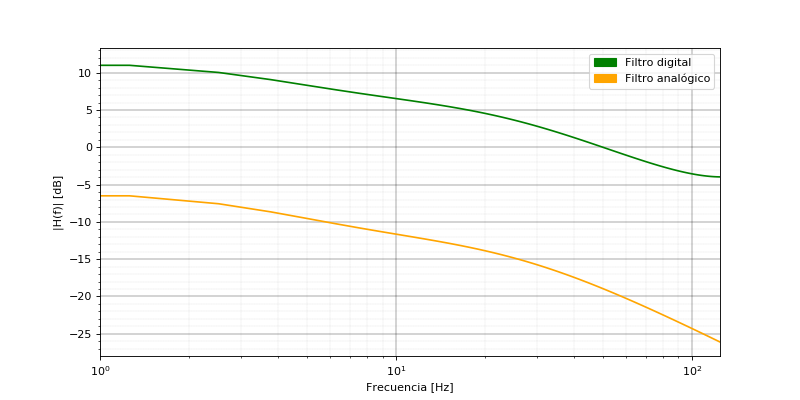
\includegraphics[width=\textwidth]
	{ej4_c.png}
	\caption{M\'etodo invariante al impulso (ejercicio 4.c)}
\end{figure}
\end{document}